\documentclass[12pt]{article} %style de document
%utilisation du squelette latex de cours de l'an dernier
\usepackage[utf8]{inputenc} %encodage des caractères
\usepackage[french]{babel} %paquet de langue français
\usepackage[T1]{fontenc} %encodage de la police
\usepackage[top=2cm,bottom=2cm,left=2cm,right=2cm]{geometry} %marges
\usepackage{graphicx} %'affichage des images
\frenchbsetup{StandardLists=true}
\usepackage{enumitem}
\usepackage{amssymb}
\usepackage{fancyhdr}
\usepackage{graphicx}
\usepackage{dsfont}
\usepackage{upgreek}


\pagestyle{fancy}
\usepackage{xcolor} %ajouter couleur de fond
\definecolor{white}{RGB}{255,255,255}
\pagecolor{white}

\usepackage{cite}


\usepackage{verbatim}

\usepackage{hyperref}

%supprimer le trait du header
\renewcommand\headrulewidth{0pt}

%supprimer les endroits de footeur et header que l'on ne veut pas
\fancyfoot[L]{}
\fancyfoot[R]{}

\fancyhead[L]{}



\begin{document} %début du document
\begin{center}


\section*{Rapport projet M1 Hacking éthique}

Titouan LE BRET

Elouan MOELLO

M1 Cybersécurité

\bigskip


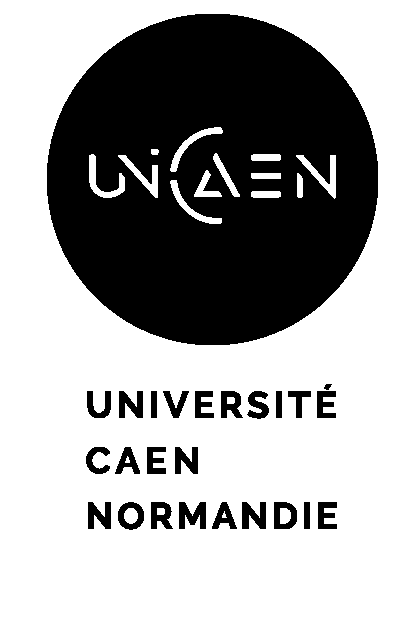
\includegraphics[scale=1.2]{images/LogoUNICAEN}
\begin{figure}[!h]
\label{}
\end{figure}
\end{center}



\newpage

\renewcommand{\contentsname}{Sommaire}
\tableofcontents




\newpage



\section{Introduction}

		Ce rapport a pour objectif de détailler la réalisation d'un projet collaboratif réalisé dans le cadre du Master 1 Cybersécurité. Nous avons fait le choix, au cours de ce projet, de réaliser deux applications différentes. Un site web développé avec Django pour la gestion d'inscriptions à une course, et une application en Rust explorant la sécurité et la validité des clés RSA. Ce rapport sera donc constitué de deux grandes parties, développant chacune un projet.
	La décision de diviser notre travail en deux projets distincts nous a semblé être une solution pertinente, nous offrant l'opportunité d'explorer à la fois une partie développement web, afin de nous former aux bonnes pratiques, tout en apprenant le langage Rust. Ce dernier est un langage très en vogue, reconnu pour sa performance, sa sécurité et sa gestion de la mémoire sans “garbage collector”.

	
			
		
	\subsection{Explications des projets}
		Le site web est conçu pour permettre à de potentiels participants de s'inscrire à une course de manière sécurisée. Il intègre des fonctionnalités de paiement en ligne, de gestion des profils utilisateurs et de visualisation du parcours de la course. Le back-end repose sur Django, quant à la partie frontend, nous avons fait au plus simple, et avons donc opté pour du HTML/CSS et quelques fonctions en javascript. Des technologies telles que OAuth ou reCAPTCHA ont été intégrées pour renforcer la sécurité et l’expérience utilisateur.

	L’application RUST est quant à elle une interface simple, permettant aux utilisateurs de tester des clefs RSA. Une page est dédiée à la validation de la clef RSA, c'est-à-dire sa conformité à différentes normes de sécurité de base. La deuxième page est réservée à l'exécution de fonctions qui testent différentes failles connues sur la partie publique des clefs RSA.

	\subsection{Objectifs de ces projets}

	Nous avons décidé de diviser notre travail en deux projets distincts, une approche qui nous a semblé pertinente pour atteindre plusieurs objectifs. D'une part, cela nous permet de nous familiariser avec le développement web, en mettant l'accent sur l'application des bonnes pratiques. D'autre part, cela nous donne l'opportunité d'apprendre le langage Rust, un langage moderne et très prisé.
	Rust se distingue par ses performances exceptionnelles, sa sécurité renforcée et sa gestion de la mémoire sans “garbage collector”. Ces qualités en font un choix privilégié pour le développement d’applications qui exigent robustesse, fiabilité et rapidité. Ces apprentissages du développement web et de Rust enrichissent nos compétences dans ces deux domaines.

	\subsection{Organisation du projet}

	Le projet initial a bien été séparé en deux gros projets, qui vont donc occuper l’ensemble des six semaines que nous avons à disposition. Nous avons choisi de prioriser le projet Django, qui était selon nous le plus intéressant à voir aboutir, la partie RUST étant quant à elle réalisée dans le but d’apprendre le langage. 
	Notre semaine était donc organisée la plupart du temps sur le format suivant : quatre jours réservés à la réalisation du projet Django, et le vendredi pouvait être consacré à l'avancée du projet RUST. Cela nous a permis de rester motivés tout au long de la durée de ce module “Hacking éthique”, en nous permettant ainsi de changer de domaine d’apprentissage au cours de la semaine.
	Pour optimiser l’organisation de ce projet, il nous a été conseillé de réaliser un diagramme de Gantt, afin de maintenir en permanence une vision globale de son avancement. Ce diagramme nous a permis de suivre les différentes étapes du projet de manière structurée et de nous assurer que chaque tâche était accomplie dans les délais impartis.


	\begin{figure}[!h]
	\begin{center}
	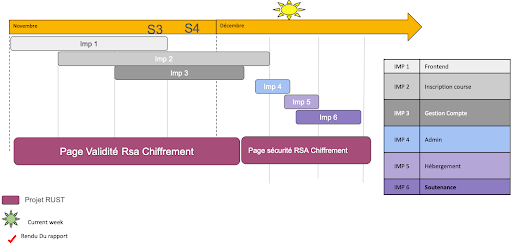
\includegraphics[scale=1]{images/diagrammeGantt}
	\caption{Diagramme de Gantt de notre projet}
	\end{center}	
	\end{figure}
	
	Il nous a ainsi été possible, au fil des semaines, de suivre et de mesurer notre avancement sur les différentes fonctionnalités que nous souhaitions implémenter. Le tableau ci-dessus présente une version simplifiée d'un tableau d'implémentation plus détaillé, dans lequel nous avons décrit les tâches spécifiques à accomplir pour mener chaque implémentation à terme. Vous trouverez ci-dessous ce tableau détaillé avec notre avancement lors de la dernière semaine du projet.
	

	\begin{figure}[!h]
	\begin{center}
		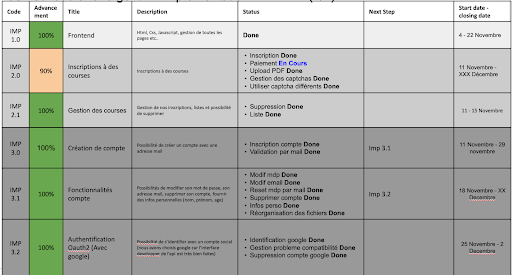
\includegraphics[scale=0.75]{images/implementation1}
		\caption{Liste des implémenatations du projet 1/2}
	\end{center}
	\end{figure}
	\begin{figure}[!h]
	\begin{center}
		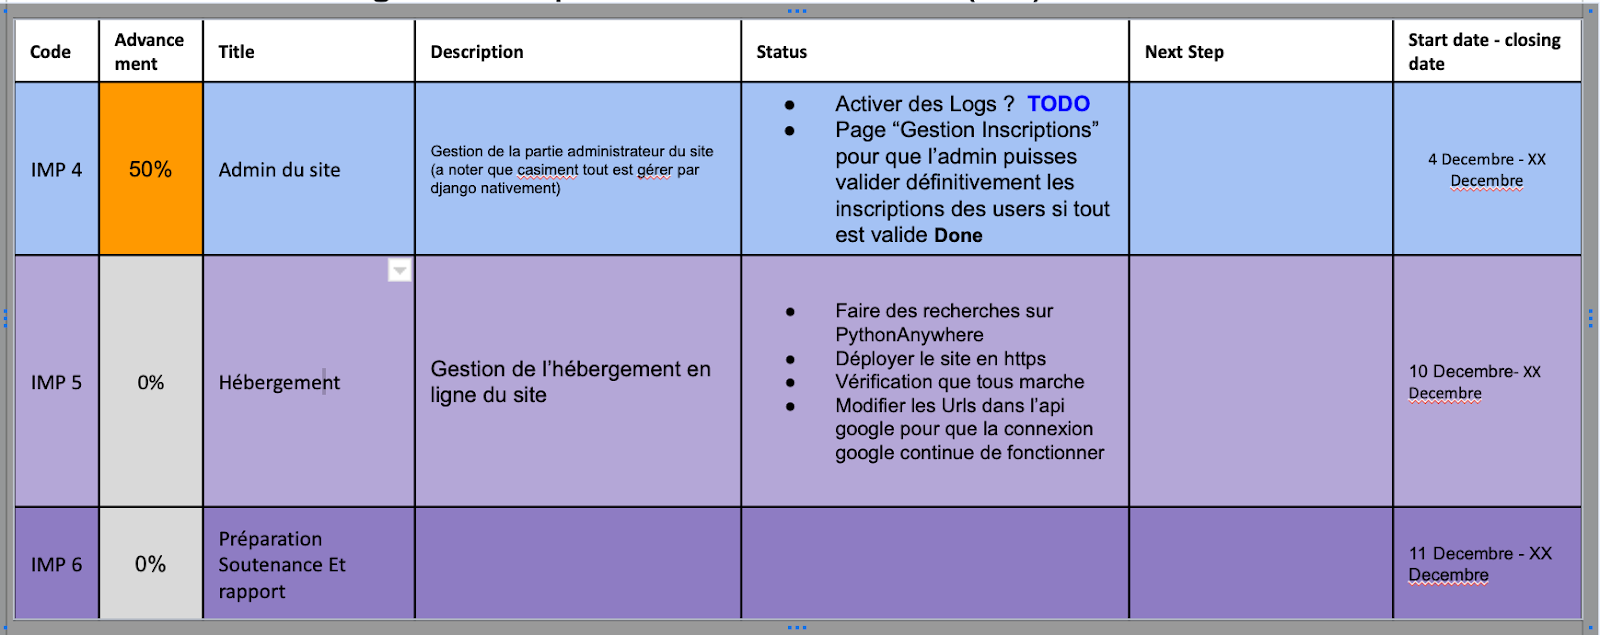
\includegraphics[scale=0.25]{images/implementation2}
		\caption{Liste des implémenatations du projet 2/2}
	\end{center}
	\end{figure}

	
	
	
\section{Conception générale}
	\subsection{Vision globale des deux projets}
		La première préoccupation que nous avons eue a été le fait d’établir une vision globale de ce à quoi nous voulions aboutir. Nous souhaitions avoir un site qui puisse accueillir de potentiels coureurs désireux de s’inscrire pour une course. Dans notre approche initiale nous voulions un système de création de compte, la possibilité de s’inscrire à une ou plusieurs courses ainsi que la possibilité de voir les différents parcours.
	Concernant le projet RUST, il fallait, selon nous que celui-ci soit très modulable, de sorte que nous puissions modifier notre vision au cours des semaines en fonction de l’avancée du projet web. 


	
	\subsection{Cahier des charges}
		\subsubsection{Le site doit donc offrir les fonctionnalités suivantes}
\textbf{\underline{Création et gestion de compte :}}
		\begin{itemize}
			\item Création de compte avec une adresse mail
			\item Suite à la création de ce compte, l’adresse email de l’utilisateur doit être vérifiée de sorte à ce que les organisateurs de la course puissent le contacter pour différentes informations. Pour ce faire, nous devons mettre en place un système d’envoi par mail d’un lien de vérification.
			\item Ajout et modification par l’utilisateur de ses informations personnelles (nom, prénom, email…).
		\end{itemize}
	
\textbf{\underline{Affichage des parcours : }}
		\begin{itemize}
			\item Affichage des différents parcours, pour permettre aux utilisateurs de les consulter avant la course.
		\end{itemize}
		
\textbf{\underline{Inscription a des courses :}}
	\begin{itemize}
		\item Inscription à une course. Les utilisateurs doivent fournir différentes informations telles que leur nom, prénom, âge, ainsi qu’une copie d’un certificat médical comme l’exige la loi.  
		\item Ce certificat doit être stocké et accessible uniquement par l’utilisateur et les administrateurs, mais surtout pas par d’autres utilisateurs du site. 
		\item Mise en place d’un système de paiement, pour que l’utilisateur puisse payer son inscription. 
		\item Possibilité pour l’utilisateur de consulter la liste de ses inscriptions et de supprimer celles-ci ou de les payer si cela n’a pas été fait précédemment.

	\end{itemize}

\textbf{\underline{Partie administrateur du site:}}

	Pour finir, nous devons gérer la partie administrateur, qui sera réservée aux organisateurs de la course,
	\begin{itemize}
		\item Possibilité de gérer les utilisateurs et leurs inscriptions. 
		\item Permettre aux administrateurs de consulter l’état du paiement de l’inscription et le certificat médical de sorte à pouvoir valider ou non celle-ci
		\item En cas de validation, une notification doit être envoyée à l'utilisateur par mail.
	\end{itemize}
	
	\subsubsection{L’application Rust Rsa}
	Comme évoqué précédemment, pour le projet d’application RSA nous n’avons pas réellement de cahier des charges fixe. Celui-ci est voué à évoluer tout au long du projet mais notre postulat de base est d’avoir : 
	\begin{itemize}
		\item Une interface graphique fonctionnelle à laquelle nous pouvons aisément rajouter des fonctions.
		\item Une page d’accueil permettant la navigation entre les pages
		\item Nous partons avec l’idée de base de créer quatre pages :
		\begin{itemize}
			\item Validité d’un clé de chiffrement RSA
			\item Sécurité d’une clé de chiffrement RSA
			\item Validité d’une signature RSA
			\item Sécurité d’une signature RSA
		\end{itemize}
	\end{itemize}
	
	
	Cependant, très vite au cours du projet nous avons révisé notre approche pour ne faire que deux pages, et nous sommes donc concentrés sur le chiffrement RSA. Ces deux pages doivent avoir les caractéristiques suivantes : 

	\begin{itemize}
		\item Entrée d’information (clé) par l’utilisateur
		\item Génération d’une clé valide, pour permettre à l'utilisateur de tester l’application facilement
		\item Vérification et conversion de ses clés
		\item Lancement des fonctions de tests par l’utilisateur
		\item Modularité pour permettre d'ajouter facilement des fonctions
	\end{itemize}


\section{Développement du site Django}
	\subsection{Fonctionnalités principales}
        Via django nous avons pu développer plusieurs fonctionnalités principales pour le projet web comme: l'inscription des utilisateurs, le paiement sécurisé via paypal, l'intégration avec OAuth2 (Google) et la sécurisation des fichiers pdf. Django permet d'implémenter une fonctionnalité administrateur, ce qui nous permet de voir les inscriptions et de les valider si toutes les informations sont correctes.


	\subsection{Approche technique}
		\subsubsection{Architecture Django :} 
            Django propose une architecture basée sur le model,view et templete.  Le dossier site course est le dossier principal, il contient le fichier setting.py qui permet de configurer les paramètres par défaut de notre application. Les autres dossiers sont des applications comme le dossiers inscriptions par exemple. Ce dossier contient des fichiers comme: \\
            - models.py:  Ce modèle stocke les informations relatives à l'inscription d'un participant à une course. \\ \\
            - view.py: Cette vue permet de faire le lien entre les tests des différentes fonctions comme l’inscription ou la suppression de l’inscription, et de faire l'appel des templetes via le fichier urls.py. Par exemple, plusieurs tests sont réalisés avant de valider l'inscription. \\ \\
            - signals.py: Ce fichier permet de gérer les signaux, par exemple lorsqu'un admin valide l’inscription d’un utilisateur, ce fichier reçoit un signal et envoie un mail de validation d'inscription à l’utilisateur grâce à une fonction.

            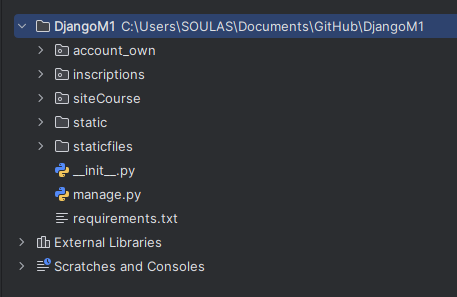
\includegraphics[scale=0.6]{images/Capture_structure.PNG}
            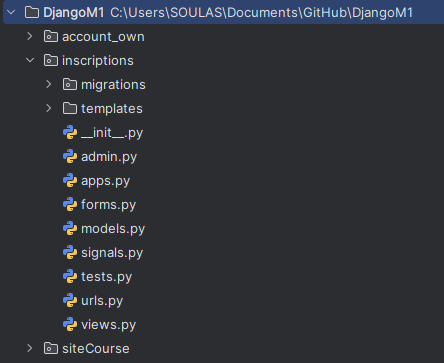
\includegraphics[scale=0.6]{images/Capture_structure-inscription.PNG}

        \subsubsection{Envoi d’e-mails :}
            Configuration de SendGrid pour des notifications fiables.\\
            L’envoi d’e-mails est utilisé dans plusieurs cas comme pour la création du compte ou pour la validation de l’inscription à une course. Voici un exemple de mail reçu lors de la validation d'une course par un administrateur.
    
            \begin{figure}[hbtp]
            \centering
            
\includegraphics[scale=0.8]{images/validationMAIL.PNG}
            \end{figure}

        \subsubsection{Protection des formulaires :}
            Chaque formulaires ont un Google reCAPTCHA qui permet de les sécuriser.
            \begin{figure}[hbtp]
            \centering
            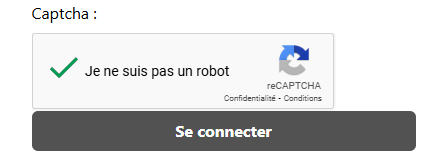
\includegraphics[scale=0.8]{images/Capture_captcha.PNG}
            \end{figure}
            
        \subsubsection{Partie administrateurs :}
            Comme évoqué précédemment nous avons une partie administrateurs qui permet de gérer toutes les inscriptions. Nous pouvons voir toutes les informations de l'utilisateur ainsi que les documents pdf importés, ce qui nous permet de vérifier la validité de celui-ci. Il y a aussi un case qui est cochée ou non si le paiement à été effectué et validé. Si toute les informations sont correctes alors l'administrateur peut cocher une case “inscription complète” qui va valider l’inscription et envoyer un mail automatiquement.

            \begin{figure}[hbtp]
            \centering
            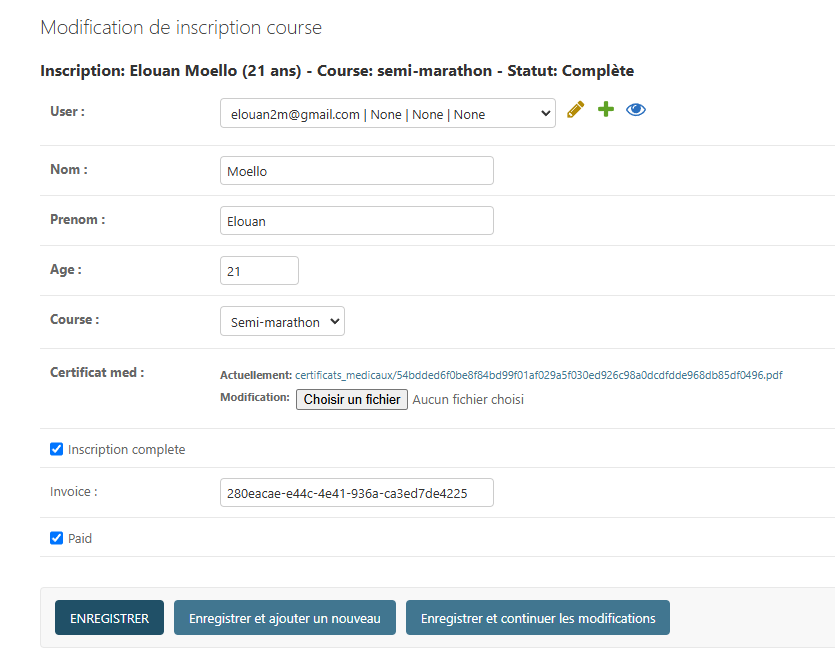
\includegraphics[scale=0.6]{images/admin_gestion.PNG}
            \end{figure}
            \newpage
        \subsubsection{Base de données :}
            Chaque inscription est stockée dans une base de données avec toutes ses informations. Ces inscriptions ont toutes un identifiant unique qui permet de les différencier. Grâce à cette BDD nous pouvons récupérer les informations voulu.


		
		
	\subsection{Sécurisation du site}
        \begin{enumerate}
            \item \textbf{Validation des données :}\\ \\
                Contrôles sur les entrées utilisateur (taille, format, validation).
            \item \textbf{Protection des fichiers :}\\ \\
                Restrictions des téléchargements non authentifiés.
            \item \textbf{Sécurisation des paiements :}\\ \\
                Le paiement est effectué grâce à l'implémentation de paypal. Lorsque l'utilisateur complète son inscription, un lien vers l’api paypal lui permet de procéder au paiement. Si l'utilisateur annule le paiement, il pourra par la suite procéder au paiement sur la page d’inscription. Sur cette page toutes les inscriptions de l'utilisateur sont affichées et il peut procéder au paiement de chaque course si celle-ci n'est pas encore payée. Pour effectuer les tests de paiement nous avons créé deux comptes paypal en mode “sand box” (bac à sable). Ces comptes sont donc fictifs et permettent d'effectuer des tests de paiement. Nous avons donc:\\
                Un compte personnel qui permet d'effectuer les paiements.\\
                personal@etu.unicaen.fr\\
                mdp: motdepasseperso\\
                Un compte business qui récupère l’argent de chaque inscription.\\
                business@etu.unicaen.fr\\
                mdp: motdepassebusiness\\
                Nous pouvons consulter ces compte avec ce lien:\\  https://www.sandbox.paypal.com/fr/home\\

        \end{enumerate}


	\subsection{Problèmes rencontrés et solutions}
        \begin{enumerate}
            \item \textbf{Difficultés techniques :}\\\\
                Configuration de SendGrid : documentation approfondie et tests successifs.\\
                Gestion des fichiers : stockage local temporaire remplacé par des solutions cloud envisagées.

            \item \textbf{Communication HTTPS et local :}\\\\
                Une fois le paiement effectué, le serveur paypal envoie un “signal ipn” qui permet de récupérer les informations de paiement. Le problème est que la communication est effectuée en https alors que notre serveur est en local lors de la phase de développement. Donc pour récupérer ce signal nous avons utilisé un outil qui est “ngrok” qui permet de mettre notre application en https. Cet outil est provisoire pour la phase de test mais ce n’est pas celui-ci qui va nous permettre à terme de mettre notre site en https.\\
                Ngrok nous permet donc d’avoir un nouveau lien en https ce qui nous permet de récupérer le signal de paiement.\\ Voici la fenêtre de gestion Ngrok.


                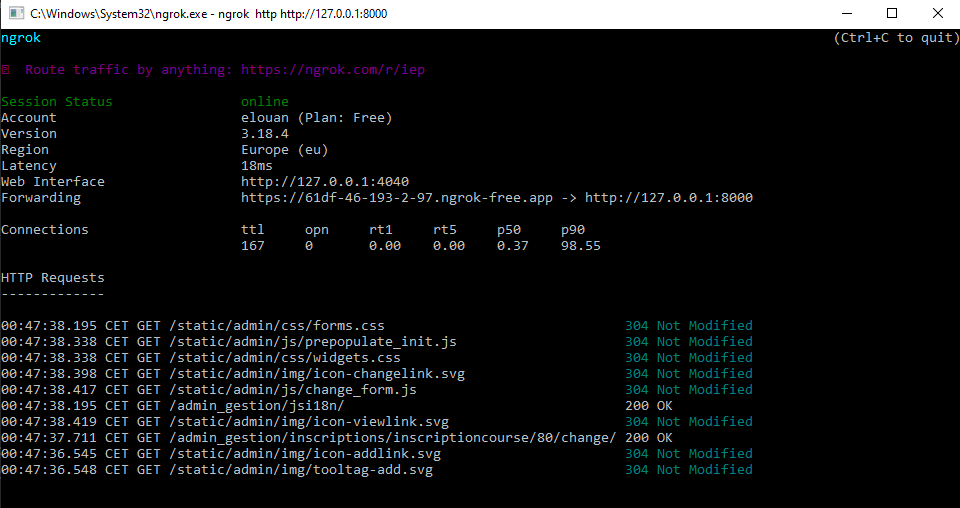
\includegraphics[scale=0.6]{images/Capture_M1Ngrok.PNG}

        \end{enumerate}
    


	\subsection{Axes d'améliorations}
		-Stockage des images en ligne (dans un DIsks sur render ou dans le CLoud google) -> demande abonnements payants \\\\
        \textbf{Paiements Stripe:}\\
            Un autre mode de paiement possible est le paiement par stripe. Il est tout aussi efficace que paypal, il intègre aussi une API. On peut dire qu’il est plus polyvalent que paypal, il intègre aussi plus de devise.
            Nous avons commencé à intégrer Stripe à notre projet web, mais vu le temps qu’il nous restait nous avons préféré nous concentrer sur la finalisation du projet.

		

	
\newpage
\section{Développement de l'application Rust RSA}
	\subsection{Objectifs et fonctionnalités principales}
		Comme précédemment évoqué, la fonction principale de cette application doit être de tester la validité et la sécurité de clés de chiffrement RSA. Cette application a été conçue pour créer un logiciel éducatif, permettant à des étudiants de tester des clés RSA pour voir si des problèmes de conformités aux normes de bases ou des failles connus sont détectées sur lesdites clés.
	C’est dans cette optique que cette application doit être simple d’usage, permettant de tester aisément plusieurs jeux de clés, et d’avoir un accès clair aux potentiels problèmes. Elle doit aussi permettre de voir son effet sans nécessairement demander à son utilisateur de chercher une clé à entrer, ainsi nous avons fait le choix d’ajouter des boutons pour générer automatiquement une clé RSA valide, pour permettre le test rapide de cette application.


	\subsection{Organisation technique}
		\subsubsection{Modélisation du projet}
		
	Pour que notre application soit simple, fonctionnelle et modulable, nous avons dû créer une architecture permissive. Ainsi, nous avons fait le choix de créer deux grands “packages” : l’un destiné au développement de l'interface graphique et l'autre à l'implémentation des différentes fonctions de tests. Nous avons choisi, pour des raisons de rapidité, de ne pas implémenter notre application sur la base d'un modèle Model-View-Controller (MVC). Pour simplifier cette implémentation, nous séparons clairement la partie Model et View dans ces deux packages, mais la partie modèle pour la sécurité des clés RSA \texttt{(safe\_enc.rs)} fait appel directement à l'interface graphique pour lui ajouter un message si le chiffré a été déchiffré.
	
Cette approche était la plus rapide pour nous permettre d’aboutir à un résultat final convaincant. En effet, cette application a été construite sur la base de tutoriels ne suivant pas le modèle MVC. Nous avons toutefois réussi à nous en rapprocher pour la partie “Validité d’une clé RSA”, mais n’avons pas eu le temps de le faire correctement pour la page “Sécurité d’une clé RSA”. Ce point de modélisation n’était pas, selon nous, une priorité. Nous avons préféré privilégier l’apprentissage du langage et le développement de l’application. En effet, les design patterns ayant déjà été abordés au cours de notre cursus de licence, nous avons estimé que cela pourrait constituer une amélioration future.

		\subsubsection{Développement de l’interface graphique}
		Nous avons choisi de développer l'interface graphique en utilisant le module “Iced”. Ce module est bien documenté et permet un développement rapide et intuitif. Une interface réactive et fluide est indispensable pour garantir une bonne expérience utilisateur, tout en assurant la robustesse et la sécurité de l'application.
		
Iced facilite la création d'interfaces multiplateformes (Windows, macOS, Linux) grâce à son architecture modulaire. Afin d’optimiser notre temps de développement et de garantir une mise en place rapide, nous avons pris la décision de garder la structure initiale du projet qui est l’implémentation de l’application en SandBox (qui était le choix fait dans l’un des tutoriels que nous avons suivi). Le choix de SandBox permet de déployer des applications simples avec une logique de base. La migration vers le trait Application aurait été nécessaire pour une gestion efficace en cas d’implémentation d’une logique asynchrone, de la nécessité de gérer plusieurs fenêtres ou encore d’interaction avec un backend.

Cette approche nous a permis de nous concentrer pleinement sur le développement de l’interface, tout en assurant une gestion fluide des interactions et des éléments visuels. Elle a été choisie pour sa rapidité d'exécution et son efficacité dans le cadre de notre projet. Nous avons pu ainsi maximiser notre productivité tout en s’assurant que l’ensemble des éléments graphiques fonctionnaient comme prévu pour être intégrés dans l'application complète.

Le fonctionnement de notre application repose donc sur cette structure qui implémente le trait SandBox. Celui-ci nous permet de développer une fonction “update”, qui repose elle-même sur l’énumération “Message”. Cette énumération représente l’ensemble des fonctions de callback que peuvent appeler nos différentes pages à la suite d’interactions utilisateurs. Voir le schéma ci-dessous, qui explique brièvement ce fonctionnement.


	\begin{figure}[!h]
		\begin{center}
			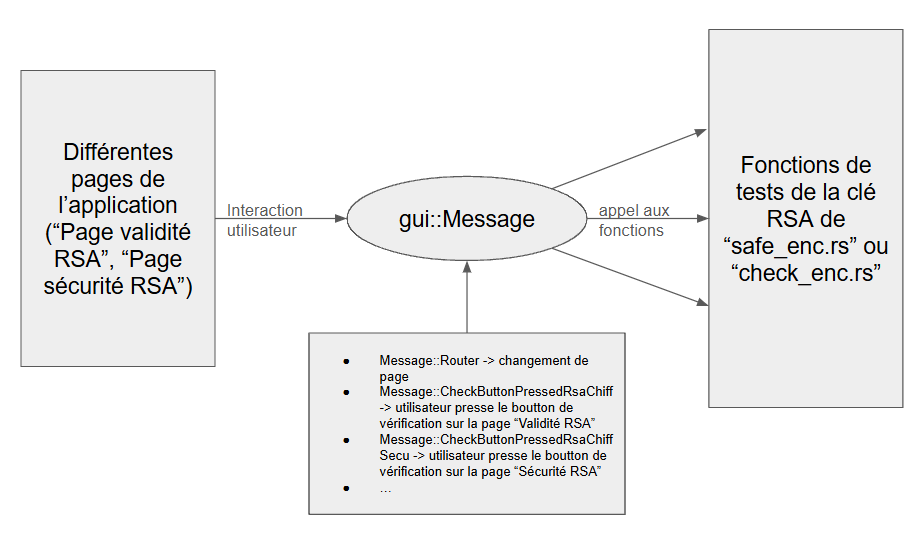
\includegraphics[scale=0.5]{images/schemaMessage}
			\caption{Fonctionnement des interactions utilisateurs}
		\end{center}
	\end{figure}

		\subsubsection{Création des fonctions de tests des clés}
		
	Le développement des différentes fonctionnalités nécessaires aux vérification des clés était un bon moyen de se familiariser avec le langage et son typage très strict. Nous avons fait des traductions des fonctions que nous avions développées au cours du premier semestre dans l’unité d’enseignement “Cryptographie”, et avons donc dû passer de Python à Rust. Cet exercice a été très instructif dans notre apprentissage, et s’est avéré plus complexe que prévu. Nous avons dû gérer certaines conversions de types ou encore certains types qui sont  gérés différemment du Python. 
		
	En parallèle, nous avons dû nous familiariser avec le module “rsa” de Rust, qui fournit des outils pour la gestion des clés RSA ainsi que pour l'implémentation de divers algorithmes cryptographiques associés. Ce module dispose d'une documentation riche et détaillée, ce qui nous a permis de rapidement comprendre son fonctionnement et de l'intégrer dans notre projet. Ce processus de découverte du module a été particulièrement formateur, car il nous a permis d'appréhender certaines spécificités de Rust, notamment sur la gestion des types et des erreurs.
	
L'un des défis majeurs que nous avons rencontrés a été de garantir la robustesse de toutes les fonctions face aux erreurs potentielles, telles que les erreurs de type ou de gestion des entrées. Cela nous a donné l'occasion de nous initier à la gestion des erreurs en Rust, et d’en comprendre le principe.


	\subsection{Problèmes rencontrés et solutions }
		\subsubsection{Gestion des entrée}
		La gestion des entrées utilisateurs a été l’un des problèmes principaux. En effet, nous devions vérifier correctement les données entrées par l’utilisateur, de sorte à ce que l’application ne soit pas interrompue si par exemple l’utilisateur venait à entrer des lettres dans les champs de texte. Ces champs de texte sont destinés à recevoir des entiers positifs, car ils vont être transformés en “BigUint”. La gestion des exceptions est donc faite sur les deux pages au moment de l'appui sur le bouton de vérification, on appelle un fonction \texttt{"validate\_inputs"}, qui va se charger de vérifier que les conversions sont possibles en les testant une à une. Si il n’y aucune erreur cette fonction renvoie “Ok”, sinon elle renvoie la liste d’erreur \texttt{(qui est un Vec<String>)}, pour que la page puisse les afficher.
		
		Cette manière de gérer les erreurs en Rust est rendu possible grâce à l'enum “Result”, décrite par le code suivant :
	
	\begin{figure}[!h]
		\begin{center}
			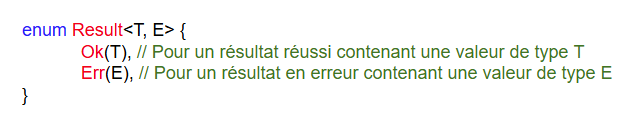
\includegraphics[scale=0.5]{images/enumResult}
			\caption{Définition de l'enum Result en Rust}
		\end{center}
	\end{figure}

		Celle-ci vient remplacer les exceptions présentes dans d’autres langages comme Java ou Python. Dans notre cas nous nous en servons de la manière suivante :
		
		\begin{itemize}
			\item S’il n’y a aucune erreur, on renvoie Ok(()) : un Ok ne contenant rien.
			\item S’il y a une ou plusieurs erreurs, on renvoie Err(errors) : une Erreur, contenant la liste des erreurs que nous avons remplies : “errors”.
		\end{itemize}
		
		
		\subsubsection{Gestion des conversions}

		Rust est un langage fortement typé, la déclaration des types est donc obligatoire. Dans certains cas, elle n’est pas faite explicitement, et c’est le compilateur qui s’en charge. Cependant, dans notre cas, nous avons rencontré quelques désagréments. Certains d’entre eux ont étaient régler sans trop de problème grâce à la documentation et des tutoriels. Mais l’un a était plus complexe. Le problème posé était la conversion de “BigUint” du module “num\_bigint”, en “BigUint” du module “rsa”. Ces deux “BigUint” sont en réalité les mêmes (“rsa” se sert de “num\_bigint”), mais d’autres modules sont fait pour fonctionner avec num\_bigint::BigUint, et donc pas avec le rsa. 
		
Nous avons donc trouver la solution de convertir notre instance de RsaBigUint en bytes (un Vecteur de “u8” (unsigned int de 8 bits)) pour ensuite construire une instance de BigUine à partir de ce vecteur.
	
	
	\begin{figure}[!h]
		\begin{center}
			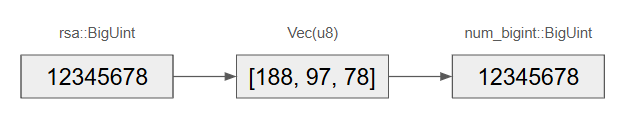
\includegraphics[scale=0.5]{images/conversionBigUint}
			\caption{Conversion de rsa::BigUint vers num\_bigint::BigUint}
		\end{center}
	\end{figure}
	
	\subsection{Résultat du rendu final}
	
	\subsection{Axes d'améliorations}






























\newpage

\section{Conclusion et perspectives}
	\subsection{Différences fondamentales}
		Objectifs distincts : site orienté utilisateur, application centrée sur la cryptographie.
Langages et environnements de développement (Python/Django vs Rust).


	\subsection{Apport de chaque projet dans le cadre de la cybersécurité}
		Impact du site : mise en œuvre des bonnes pratiques de sécurité web + apprentissage django et d’API.
Impact de l’application : exploration de la cryptographie RSA et apprentissage de RUST
	
	
	
	\subsection{Bilan global}
		Synthèse des apprentissages.
Des améliorations possibles (projets évolutifs)


\newpage
\section*{Annexes}
	\subsection{Codes sources importants}
		Extraits des parties clés de Django et Rust.
	\subsection{Ressources externes}
		Bibliographies, articles, et outils utilisés





\end{document}
